\section{How the Project Manager manages tasks}
\begin{itemize}
    \item Every PM sees the detailed project plan daily in order to be able to visualize and asses which tasks are ongoing, which deadlines are approaching and which activities are due to start. This in order to answer the questions:
        \begin{itemize}
            \item Is everything on track?
            \item What tasks are due to start?
        \end{itemize}

    \item The project manager needs to manage the work and the people.
        \begin{itemize}
            \item Are thre any open actions?
            \item Are the owners of those actions on target with their commitments?
        \end{itemize}
    
    \item When managing the work, the critical path pays an incredibly important role. 
        \begin{itemize}
            \item If the critical path is delayed the whole project will be delayed.
        \end{itemize}
    
    \item Productivity is the ration between the output and the input.
        \begin{figure}[H]
            \centering
            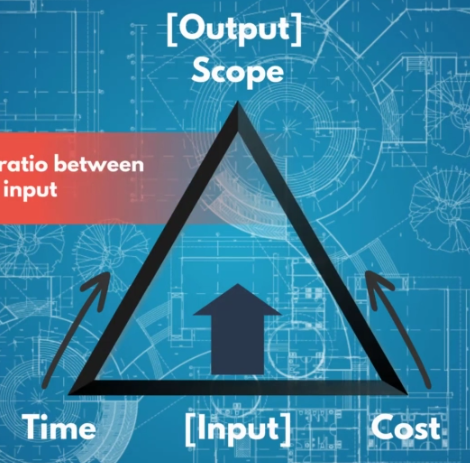
\includegraphics[width=\width\textwidth]{./figs/20221028095834.png}
            %\caption{}
        \end{figure}
        \begin{itemize}
            \item High productivity means that we have low input and high output.
        \end{itemize}
    
    \item Good productivity is almost pointless if the following activity is not ready to start.
    \item As a PM you need to constantly find ways of optimizing the workflow. But keep in mind that a good PM is only as good as their team.
    \item While the critical path is the most important, remember there are other activities and these cannot be neglected, if they are neglected they can eventually become the critical path.
\end{itemize}

%%%%%%%%%%%%%%%%%%%%%%%%%%%%%%%%%%%%%%%%%%%%%%%%%%%%%%
\section{How the Project Manager manages the team}
\begin{itemize}
    \item Communication and coordination is key for a PM when it comes to interacting with stakeholders and project team members.
    \item The PM needs to prepare the team before after and during the project.
    \item Before:
        \begin{itemize}
            \item The PM needs to prepare their team before the work begins.
            \item The PM needs to reaffirm the team member's individual responsabilities.
            \item Projects are unique and are bound to require expertise no one in the team has. In this case we need to check the possibility of hiring or giving a team member the training required to perform the activity.
            \item The PM needs to forsee the trainig or upscaleing needs and that they are addressed on time.
        \end{itemize}
    
    \item During:
        \begin{itemize}
            \item Often team members will not work together, and some team members whose activitie connect with one another will not be willing to communicate and therefore activities will be uncoordinated. The PM needs to be the one that bridges these gaps, letting the team know how their work is affecting others and who needs to finish before they can start. The PM is the mediator, problem solver, answer questions, and remove road blocks.
            \item Issues coming up is normal, but not communicating issues on time causes damage, delays and even more costs.
            \item Motivation is key, the PM must motivate their team and have honest communication with their team, have the capacity to articulate what must be done and with what purpose, as well as thank the team for good work performed and efforts expended. Building raport with a team needs to be a priority, and this will in turn augment their productivity.
            \item What happens when a team member is underperforming? The PM needs to work with the team to reach a solution together. Once a solution has been reached, they must record the agreed upon solution and the PM must improve the work, the PM must monitor the team member. If there is no improvement then the PM must examine the following options: 1. pair them with a more experienced expert to guide them, 2. reallocate work and put them on a less critial task. 
            \item Ideally, the PM must look for a solution that will not cost extra resources. Because extra resources increases the cost.
            \item Feedback and appreciation need to be given after each individual task not just when the project ends.
            \item Project updates are crucially important during the execution of the project, the stakeholders will need constant reassurance that the project is going well. During quite periods of the project is best to give updates, also giving updates when not previously asked to do so demonstrates initiative and ownership of the project.
            \item Check on the stakeholders to see if they are happy with the project so far.
            \item Its important for the stakeholders to maintain confidence in the project manager, this does not mean that PM should keep bad nes from the to create the false sense that everything is going well.
            \item The PM should be the first person to make any problems known.
            \item If the project is not on track, then the PM should communiate it immediately, because if the stakeholders hear the news from another source they will think you are not being straight forward.
        \end{itemize}
        
    \item After:
        \begin{itemize}
            \item The PM must reveal recorded information about the team such as: what they did well, what they could improve.
            \item Members of this team can eventually end up working with another project manager on another project. The PM needs to give feedback and appreciation whenever the individual merits it during and after the project.
            \item Whatever feedback you give, give it contructively. Tell them what they did well and what they could improve. And also congratulate the team.
        \end{itemize}
\end{itemize}
